\documentclass[11pt]{article}
\usepackage{amsmath}
\usepackage{amssymb}
\usepackage{graphicx}
\usepackage{tabularx}
\usepackage{fancyhdr}
\usepackage{lastpage}

% Page layout
\usepackage[top=1in, bottom=1in, left=1in, right=1in]{geometry}

% Header and footer
\pagestyle{fancy}
\fancyhf{}
\rfoot{Page \thepage}
\renewcommand{\headrulewidth}{0pt}

% Modified Question command with left-aligned number
\newcommand{\questiona}[2]{
    \noindent\textbf{Q#2.} #1 \hfill \textbf{[1 Mark]}
}

\newcommand{\questionb}[2]{
    \noindent\textbf{Q#2.} #1 \hfill \textbf{[2 Marks]}
}

\begin{document}

% Title section with horizontal line
\begin{center}
    \Large\textbf{GATE 2018 - Mining Engineering (MN)} \\
    \large\textbf{General Aptitude and Technical Questions} \\
    \rule{\textwidth}{0.5pt} % Horizontal line below heading
\end{center}

\vspace{0.5cm}

% General Aptitude Section
\section*{General Aptitude}

\questiona{“From where are they bringing their books? \_\_\_\_\_ bringing \_\_\_\_\_ books from \_\_\_\_\_.”}{1}
\begin{enumerate}
    \item[(A)] Their, they’re, there  
    \item[(B)] They’re, their, there  
    \item[(C)] There, their, they’re  
    \item[(D)] They’re, there, there  
\end{enumerate}
\vspace{0.5cm}

\questiona{“A \_\_\_\_\_\_\_ investigation can sometimes yield new facts, but typically organized ones are more successful.”}{2}
\begin{enumerate}
    \item[(A)] meandering  
    \item[(B)] timely  
    \item[(C)] consistent  
    \item[(D)] systematic  
\end{enumerate}
\vspace{0.5cm}

\questiona{The area of a square is \(d\). What is the area of the circle which has the diagonal of the square as its diameter?}{3}
\begin{enumerate}
    \item[(A)] \(\pi d\)  
    \item[(B)] \(\pi d^2\)  
    \item[(C)] \(\frac{1}{4} \pi d^2\)  
    \item[(D)] \(\frac{1}{2} \pi d\)  
\end{enumerate}
\vspace{0.5cm}

\questiona{What would be the smallest natural number which when divided either by 20 or by 42 or by 76 leaves a remainder of 7 in each case?}{4}
\begin{enumerate}
    \item[(A)] 3047  
    \item[(B)] 6047  
    \item[(C)] 7987  
    \item[(D)] 63847  
\end{enumerate}
\vspace{0.5cm}

\questiona{What is the missing number in the following sequence? 2, 12, 60, 240, 720, 1440, \_\_\_\_, 0}{5}
\begin{enumerate}
    \item[(A)] 2880  
    \item[(B)] 1440  
    \item[(C)] 720  
    \item[(D)] 0  
\end{enumerate}
\vspace{0.5cm}

\questionb{In appreciation of the social improvements completed in a town, a wealthy philanthropist decided to gift Rs 750 to each male senior citizen in the town and Rs 1000 to each female senior citizen. Altogether, there were 300 senior citizens eligible for this gift. However, only \(\frac{8}{9}\) of the eligible men and \(\frac{2}{3}\) of the eligible women claimed the gift. How much money (in Rupees) did the philanthropist give away in total?}{6}
\begin{enumerate}
    \item[(A)] 1,50,000  
    \item[(B)] 2,00,000  
    \item[(C)] 1,75,000  
    \item[(D)] 1,51,000  
\end{enumerate}
\vspace{0.5cm}

\questionb{If \(pqr \neq 0\) and \(p - x = \frac{1}{q}, \quad q - y = \frac{1}{r}, \quad r - z = \frac{1}{p}\), what is the value of the product \(xyz\)?}{7}
\begin{enumerate}
    \item[(A)] \(-1\)  
    \item[(B)] \(\frac{1}{pqr}\)  
    \item[(C)] \(1\)  
    \item[(D)] \(pqr\)  
\end{enumerate}
\vspace{0.5cm}

\questionb{In a party, 60\% of the invited guests are male and 40\% are female. If 80\% of the invited guests attended the party and if all the invited female guests attended, what would be the ratio of males to females among the attendees in the party?}{8}
\begin{enumerate}
    \item[(A)] 2:3  
    \item[(B)] 1:1  
    \item[(C)] 3:2  
    \item[(D)] 2:1  
\end{enumerate}
\vspace{0.5cm}

\questionb{In the figure below, \(\angle DEC + \angle BFC\) is equal to \_\_\_\_\_\_\_\_\_.}{9}
\begin{center}
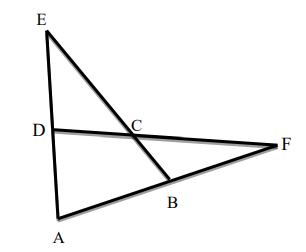
\includegraphics[width=0.5\textwidth]{figures/9.png}
\end{center}
\begin{enumerate}
    \item[(A)] \(\angle BCD - \angle BAD\)  
    \item[(B)] \(\angle BAD + \angle BCF\)  
    \item[(C)] \(\angle BAD + \angle BCD\)  
    \item[(D)] \(\angle CBA + \angle ADC\)  
\end{enumerate}
\vspace{0.5cm}

\questionb{A six-sided unbiased die with four green faces and two red faces is rolled seven times. Which of the following combinations is the most likely outcome of the experiment?}{10}
\begin{enumerate}
    \item[(A)] Three green faces and four red faces  
    \item[(B)] Four green faces and three red faces  
    \item[(C)] Five green faces and two red faces  
    \item[(D)] Six green faces and one red face  
\end{enumerate}
\vspace{0.5cm}

\section*{Technical Section}

\questiona{If \( X = \begin{bmatrix} \cos\theta & \sin\theta \\ -\sin\theta & \cos\theta \end{bmatrix} \), then \( X^T X \) is}{1}
\begin{enumerate}
    \item[(A)] \( \begin{bmatrix} 0 & 1 \\ 1 & 0 \end{bmatrix} \)
    \item[(B)] \( \begin{bmatrix} -1 & 0 \\ 0 & -1 \end{bmatrix} \)
    \item[(C)] \( \begin{bmatrix} 1 & 0 \\ 0 & 1 \end{bmatrix} \)
    \item[(D)] \( \begin{bmatrix} 0 & -1 \\ -1 & 0 \end{bmatrix} \)
\end{enumerate}
\vspace{0.5cm}

\questiona{The values of \( x \) satisfying the following condition are}{2}
\begin{center}
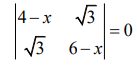
\includegraphics[width=0.2\textwidth]{figures/2.png}
\end{center}
\begin{enumerate}
    \item[(A)] 6, 4
    \item[(B)] 4, 9
    \item[(C)] 5, 6
    \item[(D)] 3, 7
\end{enumerate}
\vspace{0.5cm}

\questiona{An azimuth of \( 330^\circ \) corresponds to a quadrant bearing of}{3}
\begin{enumerate}
    \item[(A)] W60°N
    \item[(B)] N30°W
    \item[(C)] S30°W
    \item[(D)] S30°E
\end{enumerate}
\vspace{0.5cm}

\questiona{Tri-cone drill bit is a type of}{4}
\begin{enumerate}
    \item[(A)] cross bit
    \item[(B)] button bit
    \item[(C)] rotary roller bit
    \item[(D)] button drag bit
\end{enumerate}
\vspace{0.5cm}

\questiona{Exposure of weak roof in junctions of a development district in a coal mine can be decreased by}{5}
\begin{enumerate}
    \item[(A)] increasing dimension of panel barrier
    \item[(B)] stitching side walls
    \item[(C)] increasing support density at junctions
    \item[(D)] staggering the junctions
\end{enumerate}
\vspace{0.5cm}

\questiona{The property that CANNOT be determined from uniaxial compressive strength test of a rock sample fitted with strain gauges is}{6}
\begin{enumerate}
    \item[(A)] cohesion
    \item[(B)] Poisson’s ratio
    \item[(C)] modulus of elasticity
    \item[(D)] dilation
\end{enumerate}
\vspace{0.5cm}

\questiona{The radial stress concentration around a long circular tunnel excavated in rock is given by the curve}{7}
\begin{center}
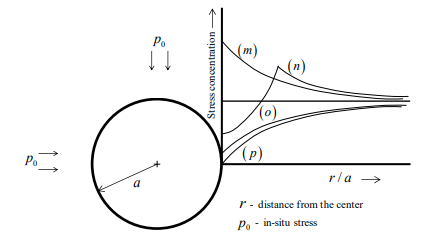
\includegraphics[width=0.5\textwidth]{figures/7.png}
\end{center}
\begin{enumerate}
    \item[(A)] m
    \item[(B)] n
    \item[(C)] o
    \item[(D)] p
\end{enumerate}
\vspace{0.5cm}

\questiona{Ward-Leonard system is provided in the winding system in order to restrict}{8}
\begin{enumerate}
    \item[(A)] over-winding of the cage
    \item[(B)] deceleration of the cage
    \item[(C)] acceleration of the cage
    \item[(D)] over-speeding of the cage
\end{enumerate}
\vspace{0.5cm}

\questiona{The equipment NOT related to extraction of coal from longwall face operation is}{9}
\begin{enumerate}
    \item[(A)] AFC
    \item[(B)] road header
    \item[(C)] powered support
    \item[(D)] DERD shearer
\end{enumerate}
\vspace{0.5cm}

\questiona{The correct figure depicting the extraction of contiguous seams in bord and pillar working is indicated by}{10}
\begin{center}
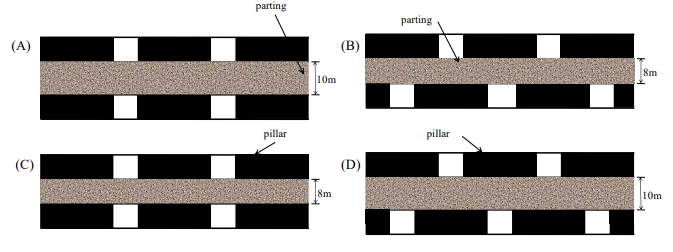
\includegraphics[width=0.7\textwidth]{figures/10a.png}
\end{center}
\begin{enumerate}
    \item[(A)] (A)
    \item[(B)] (B)
    \item[(C)] (C)
    \item[(D)] (D)
\end{enumerate}
\vspace{0.5cm}

\questiona{The significance of ‘potentially explosive mixture’ in Coward flammability diagram is -}{11}
\begin{enumerate}
    \item[(A)] leakage of fresh air may lead to explosive condition for the mixture
    \item[(B)] leakage of firedamp may lead to explosive condition for the mixture
    \item[(C)] increase in the ambient temperature may lead to explosive condition for the mixture
    \item[(D)] introduction of a source of ignition may result in explosion of the mixture
\end{enumerate}
\vspace{0.5cm}

\questiona{Considering ‘I’ as ‘intake’ and ‘R’ as ‘return’, the ventilation symbol for the shaft-bottom air-lock in a coal mine is}{12}
\begin{center}
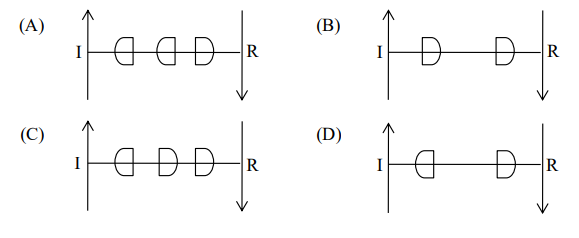
\includegraphics[width=0.8\textwidth]{figures/12.png}
\end{center}

\vspace{0.5cm}

\questiona{From a coal seam of a mine 1000 tonnes of coal is produced per day. The seam has inflammable gas emission rate of 14000 m\(^3\) per day. Percentage of inflammable gas in general body of air is 0.14. The gassiness of the seam is}{13}
\begin{enumerate}
    \item[(A)] Degree IV
    \item[(B)] Degree III
    \item[(C)] Degree II
    \item[(D)] Degree I
\end{enumerate}
\vspace{0.5cm}

\questiona{The temperature profiles and the plume patterns that are most likely to result are given in the figures. The WRONG combination is}{14}
\begin{center}
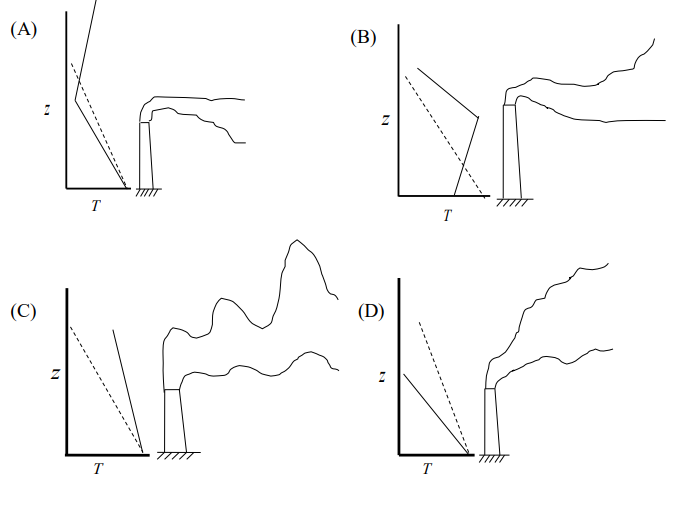
\includegraphics[width=0.8\textwidth]{figures/14.png}
\end{center}

\vspace{0.5cm}

\questiona{The inventory pattern shown does NOT represent the following.}{15}
\begin{center}
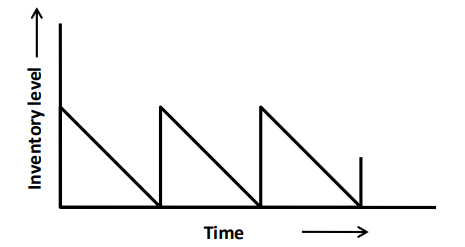
\includegraphics[width=0.5\textwidth]{figures/15.png}
\end{center}
\begin{enumerate}
    \item[(A)] Inventory is replenished instantaneously
    \item[(B)] Demand decreases with time
    \item[(C)] Shortage is not permitted
    \item[(D)] Demand is uniform
\end{enumerate}
\vspace{0.5cm}

\questiona{The figure depicts a transportation problem along with the solution. The correct statement is}{16}
\begin{center}
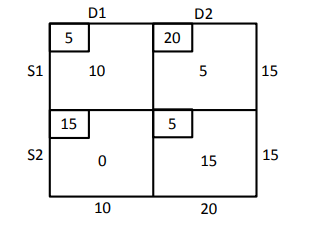
\includegraphics[width=0.5\textwidth]{figures/16.png}
\end{center}
\begin{enumerate}
    \item[(A)] unbalanced problem, optimal solution
    \item[(B)] unbalanced problem, sub-optimal solution
    \item[(C)] balanced problem, optimal solution
    \item[(D)] balanced problem, sub-optimal solution
\end{enumerate}
\vspace{0.5cm}

\questiona{The degree of the differential equation \(\frac{d^2x}{dt^2} + 3x = 0\) is \_\_\_\_\_\_\_.}{17}
\vspace{0.5cm}

\questiona{The slope of the line connecting the points (20, 6) and (40, 8) is \_\_\_\_\_\_\_.}{18}
\vspace{0.5cm}

\questiona{Two contours of RL 60 m and 70 m are separated by 34 m measured along dip of the seam. The dip of the seam in degree is \_\_\_\_\_\_\_.}{19}
\vspace{0.5cm}

\questiona{The RL of the initial station is 200 m. If \(\sum BS = 1.54\) m and \(\sum FS = 0.45\) m, then the RL of the last station in m is \_\_\_\_\_\_\_.}{20}
\vspace{0.5cm}

\questiona{For the conveyor belt drive shown, the tension on the tight side (\(T_1\)) is double that of the slack side. The coefficient of friction between belt and drum is 0.21. The minimum angle of lap (in degree) to avoid slippage of the belt is \_\_\_\_\_\_\_.}{21}
\begin{center}
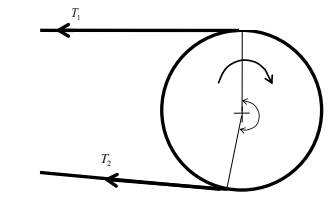
\includegraphics[width=0.5\textwidth]{figures/21.png}
\end{center}
\vspace{0.5cm}

\questiona{In a bord and pillar development district, 6 headings driven along the strike direction are surrounded by panel barriers on the dip and rise sides. The maximum possible number of faces for the panel is \_\_\_\_\_\_\_.}{22}
\vspace{0.5cm}

\questiona{A roadway in a mine, a single light source as shown, emits light uniformly in all directions. The floor level illumination at station A is 20 lux. The floor level illumination at a point B in lux is \_\_\_\_\_\_\_.}{23}
\begin{center}
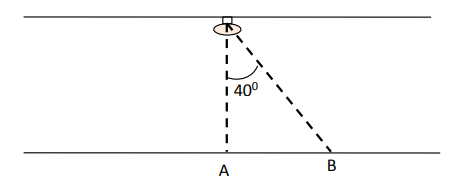
\includegraphics[width=0.5\textwidth]{figures/23.png}
\end{center}
\vspace{0.5cm}

\questiona{A system of two identical components connected in series has reliability of 0.25. The reliability of each component is \_\_\_\_\_\_\_.}{24}
\vspace{0.5cm}

\questiona{The operational status of an HEMM in a shift is shown in the diagram. The availability of the machine in \% is \_\_\_\_\_\_\_.}{25}
\begin{center}
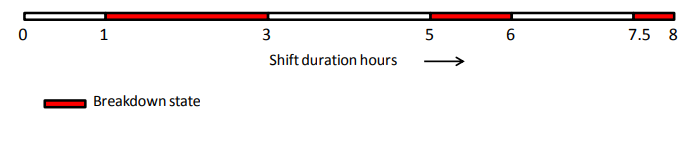
\includegraphics[width=0.8\textwidth]{figures/25.png}
\end{center}
\vspace{0.5cm}

\questionb{If \(c\) is a constant, the solution of the differential equation \(4x^2 \frac{dy}{dx} + 9y = 0\) is}{26}
\begin{enumerate}
    \item[(A)] \(81x^2 + 16y^2 = c\)
    \item[(B)] \(16x^2 + 81y^2 = c\)
    \item[(C)] \(9x^2 + 4y^2 = c\)
    \item[(D)] \(4x^2 + 9y^2 = c\)
\end{enumerate}
\vspace{0.5cm}

\questionb{Match the following blasting elements with the corresponding initiators.}{27}
\begin{tabular}{ll}
Blasting Elements & Initiators \\
P. Electric detonator & 1. Match stick \\
Q. Safety fuse & 2. Booster \\
R. Detonating fuse & 3. Exploder \\
S. Non cap-sensitive explosive & 4. Ordinary detonator \\
\end{tabular}

\begin{enumerate}
    \item[(A)] P-2, Q-3, R-4, S-1
    \item[(B)] P-3, Q-1, R-4, S-2
    \item[(C)] P-3, Q-1, R-2, S-4
    \item[(D)] P-1, Q-4, R-2, S-3
\end{enumerate}
\vspace{0.5cm}

\questionb{The following plot is developed for a rock type after a series of triaxial tests. The uniaxial compressive strength and tensile strength of the rock type, respectively, in MPa, are}{28}
\begin{center}
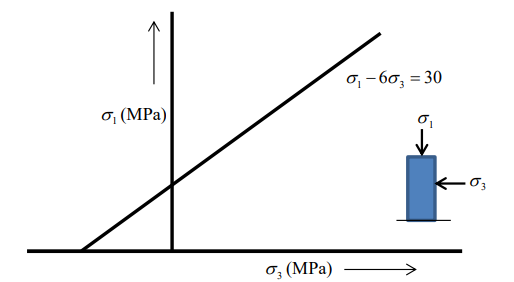
\includegraphics[width=0.5\textwidth]{figures/28.png}
\end{center}
\begin{enumerate}
    \item[(A)] 30, 5
    \item[(B)] 30, 6
    \item[(C)] 24, 6
    \item[(D)] 24, 5
\end{enumerate}
\vspace{0.5cm}

\questionb{Match the following in the context of environmental management.}{29}
\begin{tabular}{ll}
Technique & Purpose \\
P. Mulching & 1. Dust control \\
Q. Aeration & 2. Noise control \\
R. Wet-scrubbing & 3. Soil conservation \\
S. Silencer & 4. Waste water treatment \\
\end{tabular}

\begin{enumerate}
    \item[(A)] P-1, Q-4, R-3, S-2
    \item[(B)] P-3, Q-1, R-4, S-2
    \item[(C)] P-4, Q-3, R-1, S-2
    \item[(D)] P-3, Q-4, R-1, S-2
\end{enumerate}
\vspace{0.5cm}

\questionb{A panel in coal mine produces 400 tonne per day. The number of persons employed in each of the three shifts is 110, 130 and 120. As per CMR, the minimum quantity of air that needs to be circulated at the last ventilation connection of the panel in m\(^3\)/min is}{30}
\begin{enumerate}
    \item[(A)] 780
    \item[(B)] 900
    \item[(C)] 1000
    \item[(D)] 2400
\end{enumerate}
\vspace{0.5cm}

\questionb{A right conical iron ore stack on level ground of height 10 m has 60\% Fe. The height of the conical stack is extended up to 20 m using iron ore of 50\% Fe. The angle of repose of iron ore is 38\(^\circ\). The mean grade of the final stack in \% Fe is \_\_\_\_\_\_\_.}{31}
\vspace{0.5cm}

\questionb{The feasible region of a linear programming problem is shown in the figure. The maximum value of the objective function \(Z = 4X + 3Y\) is \_\_\_\_\_\_\_.}{32}
\begin{center}
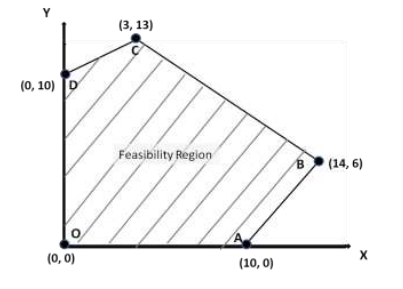
\includegraphics[width=0.5\textwidth]{figures/32.png}
\end{center}
\vspace{0.5cm}

\questionb{Cash flow of a project of duration 4 years is shown. The uniform income ‘R’, in Rs. crores, at the end of 2nd, 3rd and 4th years for an internal rate of return of 10\% is \_\_\_\_\_\_\_.}{33}
\begin{center}
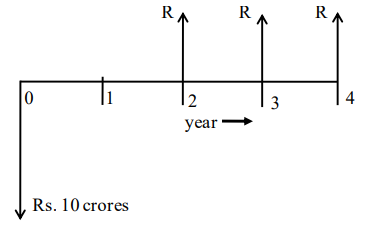
\includegraphics[width=0.5\textwidth]{figures/33.png}
\end{center}
\vspace{0.5cm}

\questionb{The grade values of alumina at three sample locations (A, B and C) in a bauxite deposit are as shown. Using the ‘inverse distance’ method, the computed grade in \% alumina at location ‘Z’ is \_\_\_\_\_\_\_.}{34}
\begin{center}
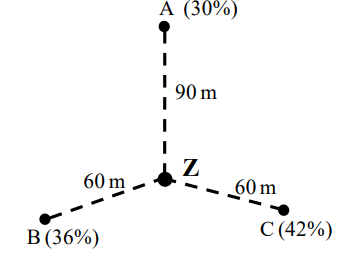
\includegraphics[width=0.5\textwidth]{figures/34.png}
\end{center}
\vspace{0.5cm}

\questionb{Economic feasibility of two methods is examined for meeting a targeted mine production. On a yearly basis, the following cost parameters (Rs in crores) are applicable for these methods:}{35}
\begin{center}
\begin{tabular}{|c|c|c|}
\hline
 & Method 1 & Method 2 \\
\hline
Fixed cost & 20 & 5 \\
Variable cost & \(2X\) & \(X^2\) \\
\hline
\end{tabular}
\end{center}
The annual rate of production, ‘X’ in million tonnes for which both the methods will yield the same operating cost is \_\_\_\_\_\_\_.
\vspace{0.5cm}

\questionb{A person standing 50 m away from an HEMM experiences 90 dB sound pressure level. If the person moves to a new location that is 70 m away from the HEMM, the sound pressure level experienced by the person, in dB, becomes \_\_\_\_\_\_\_.}{36}
\vspace{0.5cm}

\questionb{A portion of a ventilation system has two splits as shown. Split ‘A’ has a resistance of 0.2 Ns\(^2\)/m\(^8\) and a regulator of size 2.0 m\(^2\). The resistance of split ‘B’ in Ns\(^2\)/m\(^8\) is \_\_\_\_\_\_\_.}{37}
\begin{center}
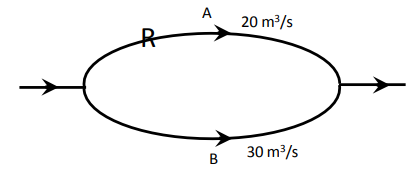
\includegraphics[width=0.5\textwidth]{figures/37.png}
\end{center}
\vspace{0.5cm}

\questionb{Air enters a bord and pillar panel at 10 ppm CO and 20.78\% O\(_2\). The air at the panel return has 80 ppm CO and 20.52\% O\(_2\). The ‘Graham’s ratio’ for the status of fire in the panel in \% is \_\_\_\_\_\_\_.}{38}
\vspace{0.5cm}

\questionb{In a sublevel stope, 20 m high excavation is made with ring drilling in a 6 m wide orebody. In an effective shift time of 6 hrs, three rings are blasted resulting in 9 m extraction length. LHDs of 5.0 m\(^3\) bucket capacity and cycle time of 5 minutes are used for ore transportation. The number of LHDs required for this operation is \_\_\_\_\_\_\_.}{39}
\vspace{0.5cm}

\questionb{A coal seam lying at a depth of 200 m is developed by bord and pillar method. Pillars are 30 m centre to centre with a gallery width of 4 m. Unit weight of the overlying strata is 28 kN/m\(^3\). If the pillar strength is 9.32 MPa, the factor of safety of pillar is \_\_\_\_\_\_\_.}{40}
\vspace{0.5cm}

\questionb{Following information about a longwall retreating panel is given:\\
Panel length = 1800 m \\
Face length = 150 m \\
Depth of web = 0.6 m \\
Shearer travels at a speed of 1.5 m/min along the face.\\
Each cutting cycle requires a non-operational time of 2 h 20 min. The panel is fully extractable.\\
The number of working days required to extract the panel is \_\_\_\_\_\_\_.}{41}
\vspace{0.5cm}

\questionb{In a direct rope haulage operating along a 1500 m long incline, 180 tonne of coal is hauled in 7 hours. The average rope speed is 7.5 km/h. The set changing time for the tubs is 2 minutes each at the top and bottom of the incline. If the tub capacity is 1.0 tonne, the number of tubs in the set is \_\_\_\_\_\_\_.}{42}
\vspace{0.5cm}

\questionb{An SDL of 1.0 tonne capacity operates with a cycle time of 6 minutes. The dimension of the face is 4 m x 3 m. Five blasts are conducted per shift with an average pull of 1.2 m. If the density of blasted coal is 0.8 tonne/m\(^3\), the time required by the SDL in the shift to lift all the prepared coal in hours is \_\_\_\_\_\_\_.}{43}
\vspace{0.5cm}

\questionb{A force diagram is shown below. Considering clockwise moments to be positive, the resultant moment about A in Nm is \_\_\_\_\_\_\_.}{44}
\begin{center}
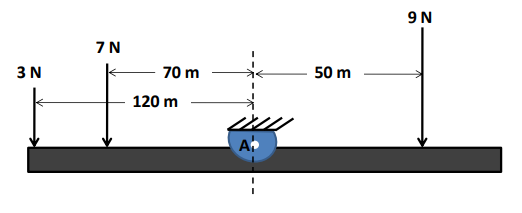
\includegraphics[width=0.5\textwidth]{figures/44.png}
\end{center}
\vspace{0.5cm}

\questionb{The experiment to determine permeability of a soil sample is illustrated below. The cross-sectional area of the sample is 20.0 cm\(^2\). The permeability of the soil sample in cm/s is \_\_\_\_\_\_\_.}{45}
\begin{center}
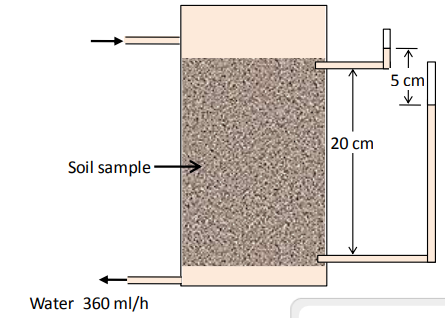
\includegraphics[width=0.5\textwidth]{figures/45.png}
\end{center}
\vspace{0.5cm}

\questionb{In underground face blasting, the pull is found to be 10\% less than the drillhole length. The headings of 3.6 m width are supported by prop density of 1.44/m\(^2\). The hole length is 1.5 m, and 6 rounds of blasting are done in the panel per shift. The number of props to be erected in a shift is \_\_\_\_\_\_\_.}{46}
\vspace{0.5cm}

\questionb{The immediate roof of a mine is supported by bolts of length 1.5 m, arranged in 1.2 m x 1.2 m grid pattern. If the unit weight of roof rock is 2.25 tonne/m\(^3\) and load carrying capacity of each bolt is 7.5 tonne, the factor of safety of the support system is \_\_\_\_\_\_\_.}{47}
\vspace{0.5cm}

\questionb{In a level terrain, a vertical orebody of 20 m uniform width is worked by surface mining method. The density of the ore is 2.5 tonne/m\(^3\). The ultimate pit has a depth of 60 m, width of 20 m at pit bottom, and a pit slope of 45\(^\circ\). The overall stripping ratio for this condition in m\(^3\)/tonne is \_\_\_\_\_\_\_.}{48}
\vspace{0.5cm}

\questionb{A 20 m long steel tape used for survey is found to be short by 10 cm. If the area measured with the steel tape is 5000 m\(^2\), the actual area in m\(^2\) is \_\_\_\_\_\_\_.}{49}
\vspace{0.5cm}

\questionb{The following figure shows the designed blast pattern of a bench. The explosive column is charged at 18 kg/m. If the unit weight of the blasted material is 2.5 tonne/m\(^3\), the powder factor for the blast in tonne/kg is \_\_\_\_\_\_\_.}{50}
\begin{center}
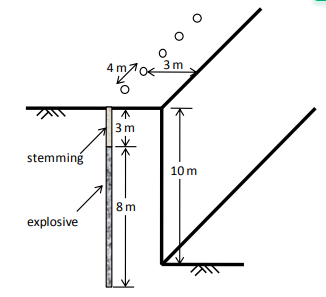
\includegraphics[width=0.5\textwidth]{figures/50.png}
\end{center}
\vspace{0.5cm}

\questionb{Two points on the equator have longitudes 55\(^\circ\)E and 25\(^\circ\)W. Considering radius of Earth as 6400 km, the distance between the two points in km is \_\_\_\_\_\_\_.}{51}
\vspace{0.5cm}

\questionb{Sum of the series 5, 10, 15, ……….., 500 is \_\_\_\_\_\_\_.}{52}
\vspace{0.5cm}

\questionb{The sample standard deviation for the following set of observations is \_\_\_\_\_\_\_.\\
40, 45, 50 and 55}{53}
\vspace{0.5cm}

\questionb{For the given function \(f(x, y) = (x + 3)(y + 4)\), the value of \(\frac{\partial f}{\partial x} + \frac{\partial f}{\partial y}\) at \(x = 2\) and \(y = 1\) is \_\_\_\_\_\_\_.}{54}
\vspace{0.5cm}

\questionb{Given \(y = x^2 + 6x + 6\), the value of \(\frac{d}{dx} (\ln y)\) at \(x = 2\) is \_\_\_\_\_\_\_.}{55}
\vspace{0.5cm}

\vspace{5cm}
\begin{center}
\textbf{END OF THE QUESTION PAPER} \\
\rule{\textwidth}{0.5pt}
\end{center}

\end{document}
